\documentclass{beamer}

\usepackage[spanish]{babel}
\usepackage[utf8]{inputenc}
% Vary the color applet  (try out your own if you like)
\colorlet{structure}{red!65!black}

\usepackage{beamerthemesplit}
\usepackage{graphics}
\usepackage{graphicx}
\usepackage{hyperref}
\usepackage{array}

\def\imagetop#1{\vtop{\null\hbox{#1}}}
\newcommand{\bigO}{\mathcal{O}}

\usepackage[autoplay, loop,controls]{animate} 
\usepackage{movie15}
\usetheme{Madrid}

\title{HML - A Machine Learning Library in Haskell}

\begin{document}
\date{}
\author{Hancel González y Kelwin Fernández}
\frame
{
    \maketitle
}

\frame
{
	\frametitle{HML}
	
	\begin{itemize}
		\item Librería de aprendizaje de máquina implementada en Haskell.
		\item Que aproveche el paralelismo natural de estos algoritmos.
		\item Algoritmos y Máquinas implementados\pause \ldots por ahora
		\pause
		
		\begin{itemize}
		\item Regresión Lineal.
		\item Regresión Logística.
		\item Máquina de Soporte de Vectores.
		\item Redes Neuronales y Backpropagation.
		\item K-Means
		\end{itemize}
	\end{itemize}
}

\frame{
	\frametitle{Regresión Lineal}
	
	\begin{center}
	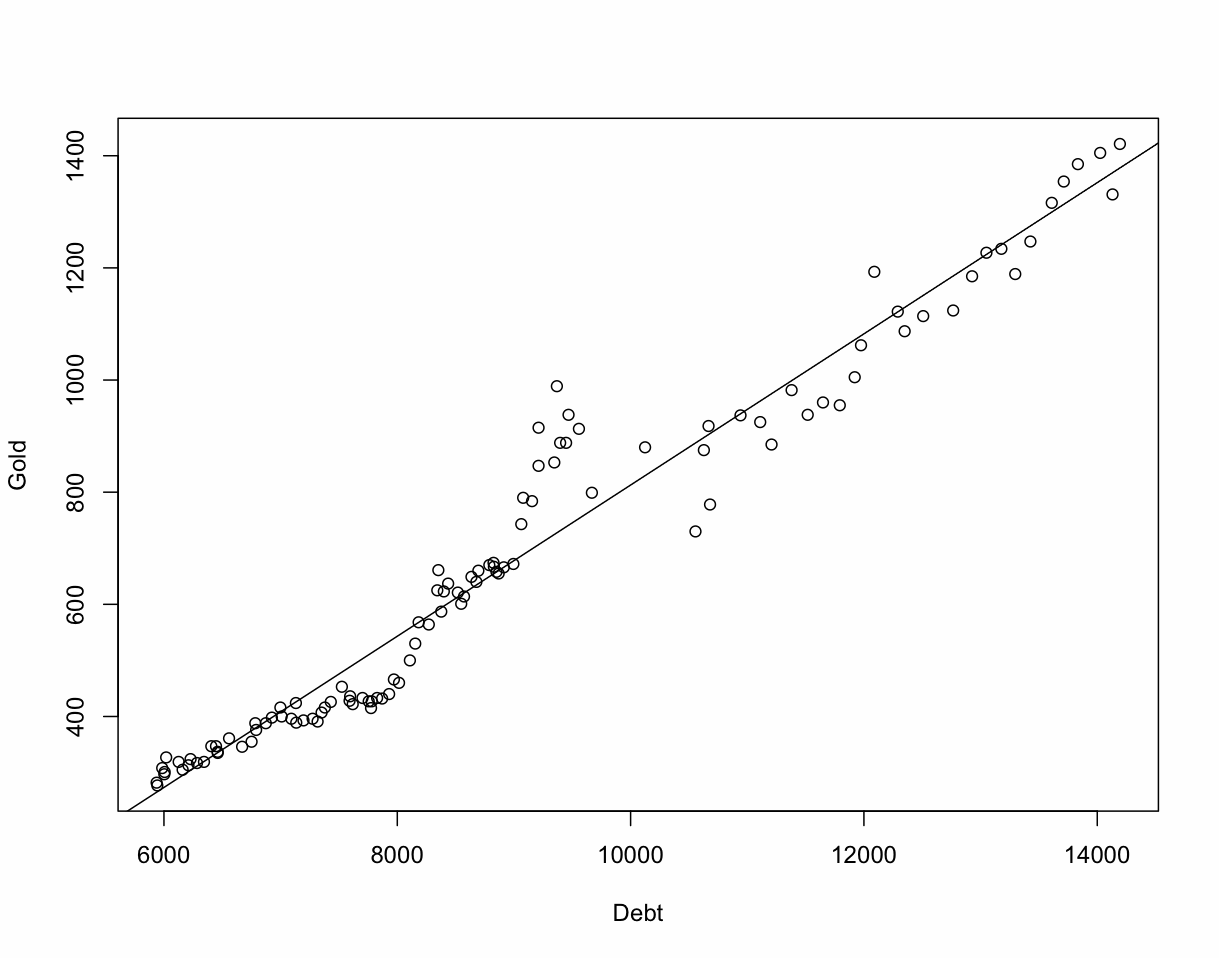
\includegraphics[width=0.8\textwidth]{figures/linear_regression.png}
	\end{center}
}

\frame{
	\frametitle{Regresión Lineal - Aspectos de Interés}
	
	\begin{itemize}
	\item Uso de la combinación de los Monads Reader, Writer y State
	para configuración de los experimentos, estadísticas de progreso
	de aprendizaje y la máquina mutable.
	\item Paralelismo mediante \texttt{Control.Parallel}.
	\item Uso de la librería \texttt{hmatrix} de álgebra lineal.
	\item Uso de la librería adicional \texttt{gnuplot} para
	la graficación del progreso de aprendizaje.
	\item Algoritmos de entrenamiento mediante \textit{gradient descent}
	y \textit{normal equation}.
	\end{itemize}
}

\frame{
	\frametitle{Regresión Lineal - Ejemplo de Uso}
	
	
}

\frame{
	\frametitle{Redes Neuronales}
	
	\begin{itemize}
	\item Combinador RWS análogo a los anteriores.
	\item Paralelismo mediante anotaciones.
	\item Algoritmo de Aprendizaje: \textit{Stocasthic Backpropagation}.
	\end{itemize}
	
	\begin{center}
	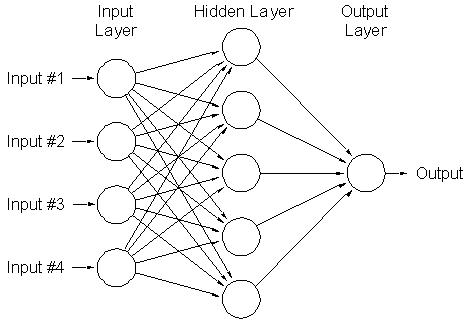
\includegraphics[scale=0.4]{figures/ann.png}
	\end{center}
}

\frame{
	\frametitle{Redes Neurales - Ejemplo de Uso}
}

\frame{
	\frametitle{K-Means}
	
	\begin{itemize}
	\item Algoritmo de aprendizaje no supervisado.
	\item Agrupación de datos identificando patrones.
	\end{itemize}
	
	\begin{center}
	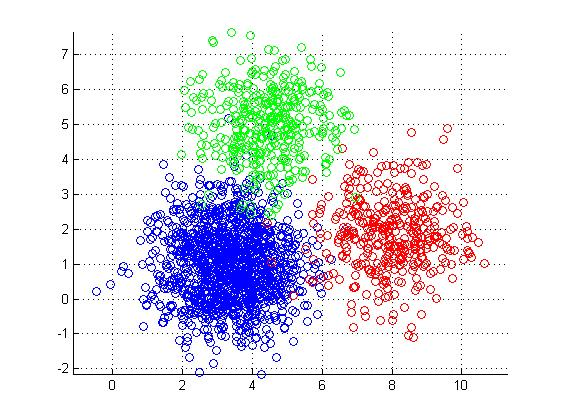
\includegraphics[scale=0.4]{figures/kmeans.jpg}
	\end{center}
}

\frame{
	\frametitle{K-Means - Algoritmo}
	
	\begin{enumerate}
	\item Crear K centroides aleatorios.
	\item Asignar a cada punto su centroide más cercano.
	\item Mover cada centroide a su centro de masa.
	\item Repetir los pasos 2 y 3 hasta converger.
	\end{enumerate}
	
	Paralelización de los pasos 2 y 3, recalculando cada
	centroide partiendo los datos de entrada en grupos y
	uniendo finalmente.
}

\frame{
	\frametitle{K-Means - Ejemplo de Uso}
	
	\begin{enumerate}
	\item Comprimir imágenes.
	\item Agrupar los píxeles en $k$ grupos, asignar a cada
	píxel el color que mejor los represente a todos (el centroide, dah!).
	\item Necesario $log(k)$ bits para representar cada píxel.
	\item Para 16 colores, se reduce el almacenamiento de $24$ bits
	por píxel (RGB) a 4 bits.
	\end{enumerate}
	
	Problema: no se ha encontrado una librería buena para procesamiento
	de las imágenes en 6.12. Actualmente se realiza con \textit{OpenCV}
	en C++.
}

\frame{
	\frametitle{K-Means - Ejemplo de Uso (Imagen Original)}
	
	\begin{center}
	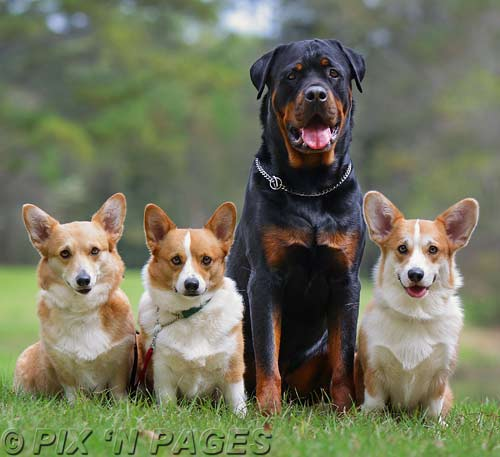
\includegraphics[width=7cm,height=7cm]{figures/kmeans/rott.png}
	\end{center}
}

\frame{
	\frametitle{K-Means - Ejemplo de Uso (10 iteraciones después)}
	
	\begin{center}
	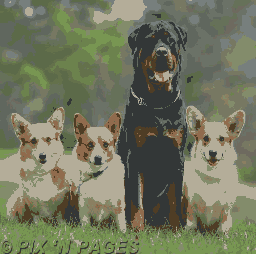
\includegraphics[width=7cm,height=7cm]{figures/kmeans/rottAndCorgies10.png}
	\end{center}
}

\frame{
	\frametitle{K-Means - Ejemplo de Uso (50 iteraciones después)}
	
	\begin{center}
	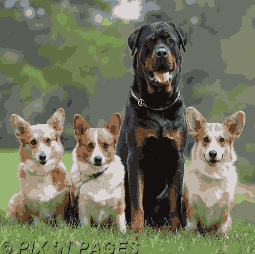
\includegraphics[width=7cm,height=7cm]{figures/kmeans/rottAndCorgies50.png}
	
	\bigskip
	N2 (32 seg), N1 (44 seg)
	\end{center}
}

\frame{
	\frametitle{K-Means - Ejemplo de Uso}
	
	\begin{center}
	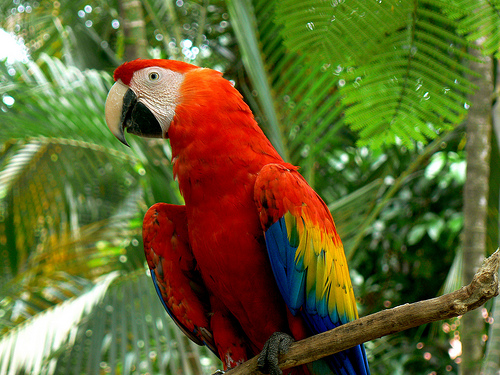
\includegraphics[width=5cm,height=5cm]{figures/kmeans/guacamaya.png}
	
	\bigskip
	Antes
	\end{center}
}

\frame{
	\frametitle{K-Means - Ejemplo de Uso}
	
	\begin{center}
	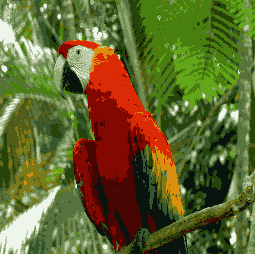
\includegraphics[width=5cm,height=5cm]{figures/kmeans/o_guacamaya.png}
	
	\bigskip
	Después
	\end{center}
}

\frame{
	\frametitle{K-Means - Ejemplo de Uso}
	
	\begin{center}
	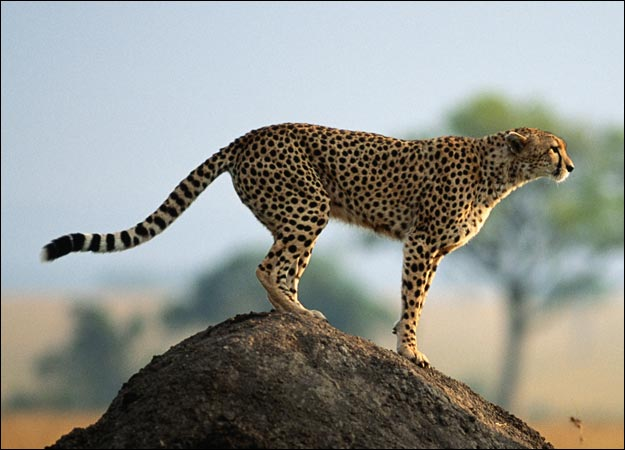
\includegraphics[width=5cm,height=5cm]{figures/kmeans/cheetah.jpg}
	
	\bigskip
	Antes
	\end{center}
}

\frame{
	\frametitle{K-Means - Ejemplo de Uso}
	
	\begin{center}
	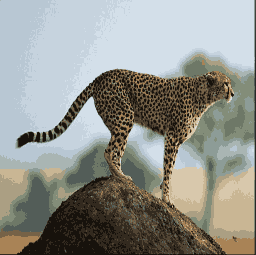
\includegraphics[width=5cm,height=5cm]{figures/kmeans/cheetah_out.png}
	
	\bigskip
	Después
	\end{center}
}

\frame{
	\frametitle{K-Means - Ejemplo de Uso}
	
	\begin{center}
	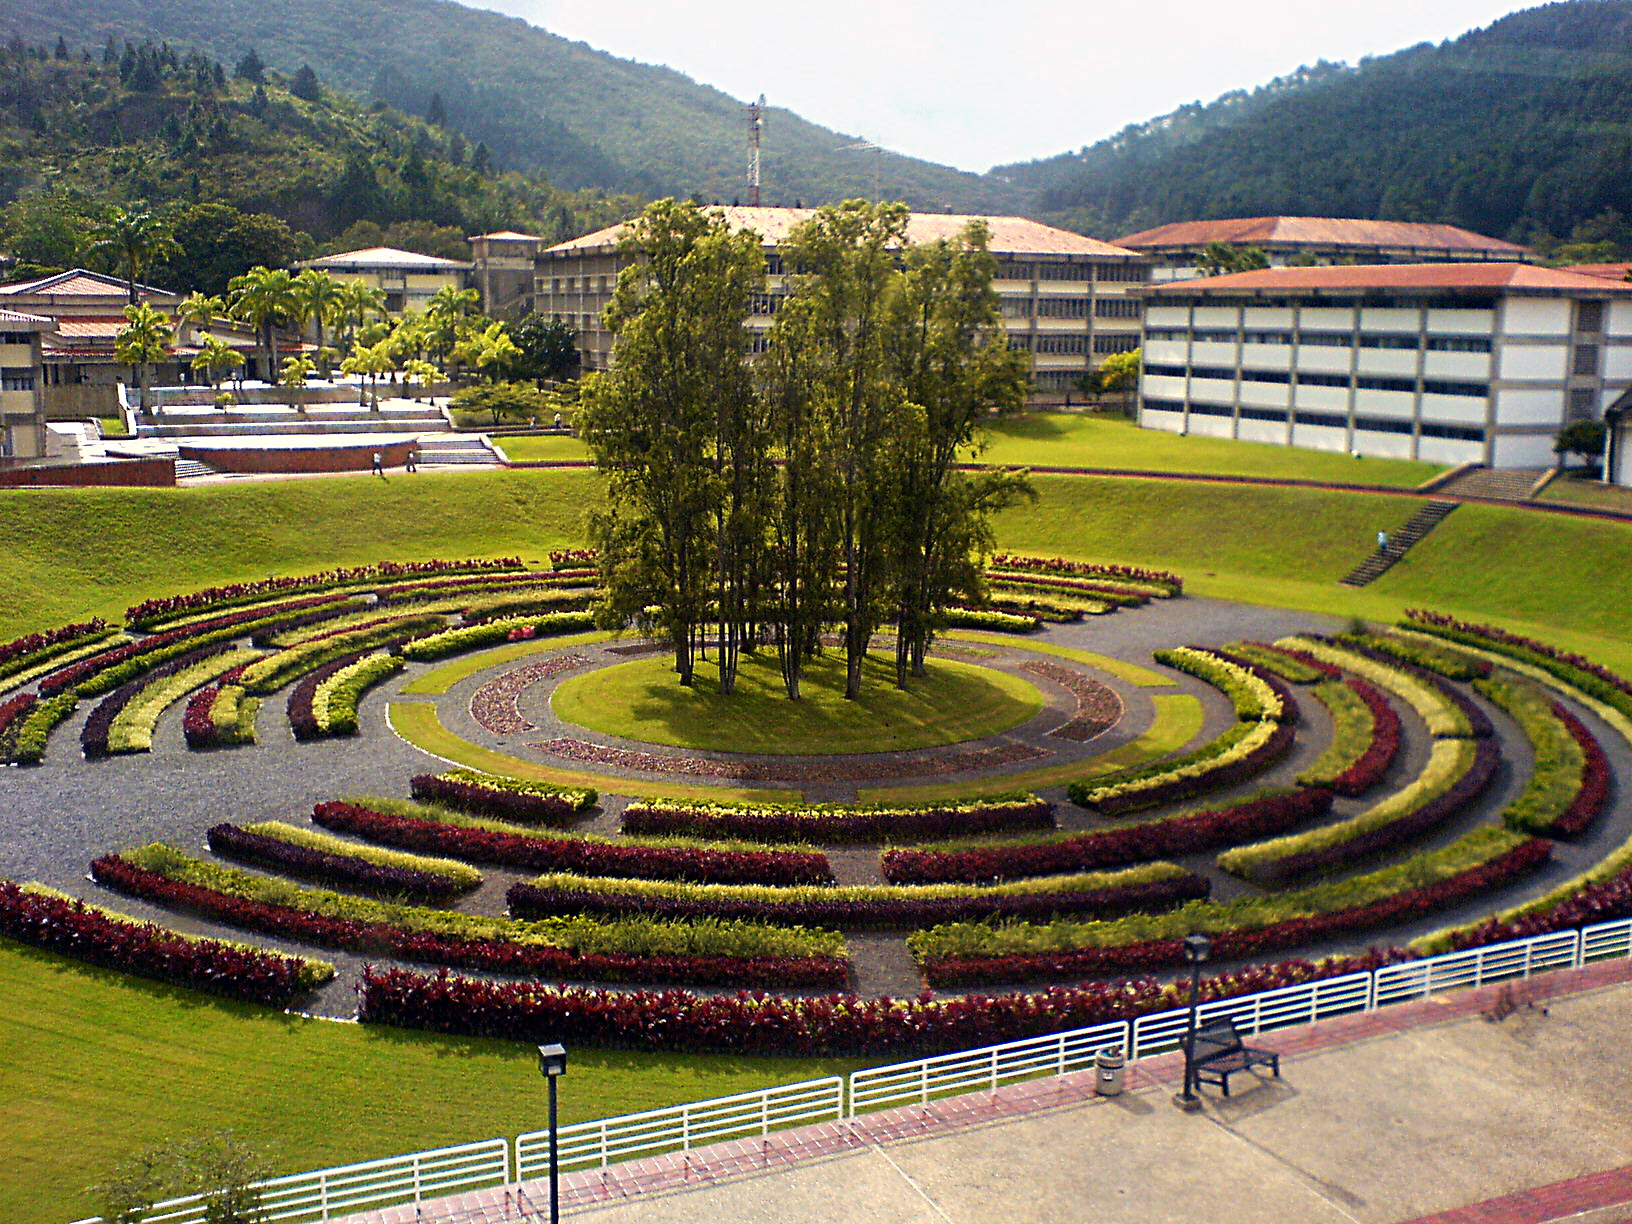
\includegraphics[width=5cm,height=5cm]{figures/kmeans/cromovegetal.jpg}
	
	\bigskip
	Antes
	\end{center}
}

\frame{
	\frametitle{K-Means - Ejemplo de Uso}
	
	\begin{center}
	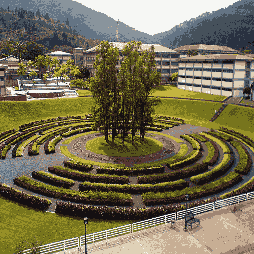
\includegraphics[width=5cm,height=5cm]{figures/kmeans/o_cromovegetal.png}
	
	\bigskip
	Después
	\end{center}
}

\frame{
	\frametitle{K-Means - Ejemplo de Uso}
	\begin{center}
	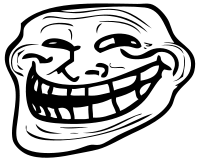
\includegraphics[width=5cm,height=5cm]{figures/kmeans/trollface.png}
	
	\bigskip
	Antes
	\end{center}
}

\frame{
	\frametitle{K-Means - Ejemplo de Uso}
	\begin{center}
	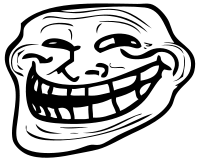
\includegraphics[width=5cm,height=5cm]{figures/kmeans/trollface.png}
	
	\bigskip
	Después
	\end{center}
}
\end{document}